%!TEX root = manual_booklet.tex

\begin{center}
   {\colorbox{grey2}{
         \begin{minipage}[t]{0.9\textwidth}
The tutorial presented here is a tutorial on the use of PsN,
Xpose, and Pirana combined, and has been published before (\textit{\small Modeling \& 
simulation workbench for NONMEM: tutorial on Pirana, PsN and Xpose; Keizer RJ, Karlsson MO, Hooker AC}\normalsize, CPT-PSP 2013). 
The tutorial provides an excellent introduction to Pirana's basic
functionality, and its connections to the other tools. This
tutorial is aimed at modelers that have some familiarity
with NONMEM, but have no or limited experience with PsN or Xpose. The
training material and solutions are available from the Pirana website, or from CPT-PSP.
          \end{minipage}
      }
   }
\end{center}

\section{Introduction}
Several software tools are available that
facilitate the use of the NONMEM software and extend its
functionality. This tutorial shows how three commonly used and freely
available tools, Pirana, PsN, and Xpose, form a tightly integrated
workbench for modeling \& simulation with NONMEM. During the tutorial,
we provide some guidance on what diagnostics we consider most useful
in PK model development, and how to construct them using these
tools. 

\section{Background}Started in the early 80s with the development
of the NONMEM (acronym based on “NON-linear Mixed-Effects Modeling”)
software[1], “population analysis” has proven to be extremely useful
within pharmacometrics, both in the development of new drugs[2] and
the improvement of therapy with approved drugs.[3] Development of the
NONMEM software continues, and, although over time several other
modeling software tools have become available, NONMEM is still
regarded as the gold standard within the pharmacometric community: a
recent survey identified NONMEM (together with PsN[4]) as the most
frequently used software tool by far.[5] Modeling and simulation in
clinical pharmacology, and the use of NONMEM in particular, however,
has a steep learning curve for most starting researchers. This is
partially due to the fact that NONMEM is invoked from the command
line, and models are implemented using a Fortran-derived syntax
(NM-TRAN). Additionally, at its core, NONMEM performs only model
estimation (or simulation), and the implementation of essential
diagnostic tools such as bootstrap analyses and the creation of
goodness-of-fit plots are left to the modeler. Therefore, alongside
the development of NONMEM, many third-party tools have been developed
that facilitate the use of NONMEM by providing tools for organization
and automation. In this tutorial we will demonstrate the use of some
of the most widely used auxiliary software tools: PsN, Xpose[6], and
Pirana[7]. All three tools are released under an open source license
and are freely available (except for the commercial use of Pirana, for
which a commercial license is required). Separately, each tool offers
useful functionalities, but there is a synergistic benefit as well
when used together. 

The aim of this tutorial is to show how these three tools provide a
comprehensive workbench for modeling and simulation. This will be done
by showing examples of the most often encountered steps in PK model
development, i.e. a covariate modeling procedure and model evaluation
using residual- and simulation-based diagnostics. However, the aim of
the tutorial is not to provide guidance on how to perform a population
PK analysis, but strictly on these software tools. A detailed overview
of important aspects in population PK analyses has recently been
presented in this journal, and we refer the reader to that article for
guidance.[8] The current tutorial is structured in three parts: first
a brief introduction to these software tools is given, explaining
their basic purpose. In the main part of the tutorial, we show how a
typical PK model building analysis is performed with these tools and
NONMEM. At the end of the tutorial, several interesting additional
features are highlighted for each specific tool. We will assume the
reader is already somewhat familiar with NONMEM, although we have made
efforts to present and discuss the tools in a general fashion where
possible. All of the presented models, datasets, output, and
diagnostic plots are available in the online
materials.

\subsubsection{Software}
In this tutorial we will use NONMEM 7.2, Pirana
2.7.0, PsN 3.5.3, and Xpose 4.3.5. It is likely that future versions
will behave similarly, but in earlier versions not all functions
presented here may be available. We will show screenshots taken from
Windows, but all programs discussed here function similarly on all
major operating systems.

\begin{description}

\item [NONMEM] [9] is modeling software that allows the user to estimate
parameters in mixed-effects models (“population approach”) based on
maximum likelihood- or Bayesian techniques that use either gradient or
stochastic estimation methods. NONMEM translates model code written in
a unique Fortran-based syntax (NM-TRAN) into pure Fortran code, which
is then compiled and executed. NONMEM is currently developed by ICON
Development Solutions under a proprietary software license.

\item[PsN] [4] is a combination of tools for performing advanced modeling \&
simulation (M\&S) with NONMEM. It allows the implementation of
bootstraps, visual predictive checks and many other useful
functionality. PsN is written in Perl (and needs Perl installed,
freely available for all major operating systems), and is operated
from the command-line. Development started in 2000, and updates have
been released with regular intervals.

\item[Xpose] [6] is a tool for plotting and analyzing NONMEM output,
developed as a module for the R software (http://cran.r-project.org/,
open source, S-based statistical software). The tools in Xpose can be
used from the R command line or from a text-based menu system in
R. Xpose was first released in 1998, and was initially developed for
S-Plus. The current version (main version number 4) is however
released exclusively for R and builds upon the lattice module for
plotting. Both PsN and Xpose are developed at Uppsala University and
are released under an open-source license (GNU v2).

\item[Pirana] [7] is a graphical user interface for NONMEM, PsN and
Xpose/R. It has functionality for model management, model execution,
output generation, interpretation of results, and includes many other
tools. Development of Pirana started in 2007 at the Netherlands Cancer
Institute / Slotervaart Hospital (Amsterdam, NL), and is currently
continued by Pirana Software \& Consulting BV
(http://www.pirana-software.com). Pirana is released under an open
source license (Creative Commons) for academic users as well as a
commercial license. 

\end{description}

\section{Tutorial}In this tutorial, file and folder names are shown
in \fname{italic}, Pirana actions are shown \action{red-italic}, while commands,
arguments, NONMEM syntax and screen output are shown in \command{fixed-width
font}. We will step through an example model building exercise, with
the intent of showing how to create, manage, and evaluate
pharmacokinetic (PK) models for a given dataset. The PK dataset used
in this tutorial (\fname{pktab1}) is available in the on-line material, and
contains plasma concentration data obtained from a simulated clinical
trial of a novel iv drug, performed in 50 patients, measured at 8 time
points. All model files that are mentioned in this article are also
available on-line and can be used as reference. Make sure that all
software is installed correctly, and NONMEM runs can be started from
both PsN and Pirana (visit the respective websites for installation
instructions), and that the Xpose4 package is installed in R. Create a
folder for this analysis somewhere on your hard-drive, and put \fname{pktab1}
in this folder. Browse to this folder in Pirana, and save it as the
project “TutorialPSP” (\action{button 4 in figure 1}). As starting point for
NONMEM models, it is often easiest to use the PK model wizard in
Pirana, or start from one of the models available in the model
library. Start the wizard dialog window in Pirana (\action{Tools $\rightarrow$ Wizards})
and choose the PK model wizard, and explore the options. However, for
this tutorial we have already provided the first model (run1.mod):
copy the model run1.mod from the online material to the folder you
created. This model should now be visible in the Pirana main model
list when you direct Pirana to the right folder (if not, refresh
\action{Pirana button 5 in figure 1}). 

\begin{figure}[H] \centering
    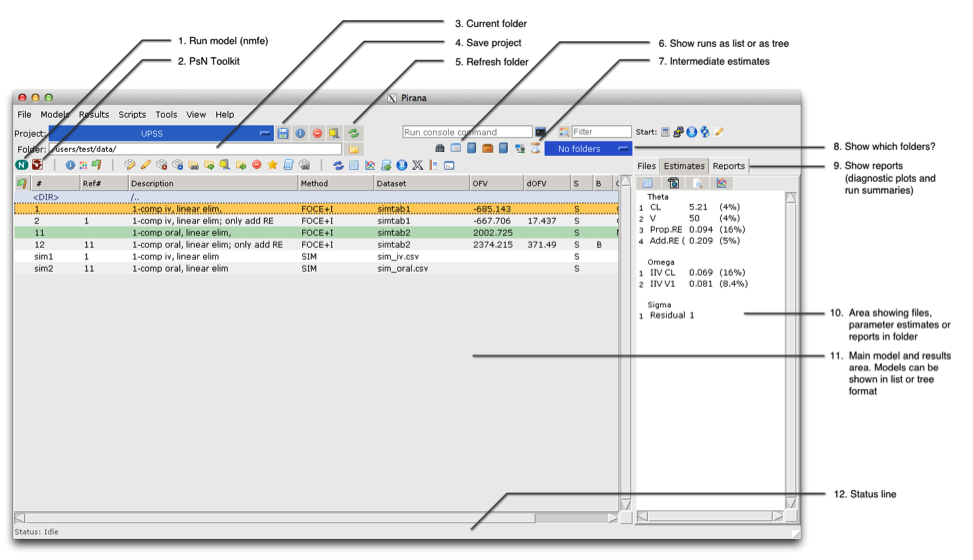
\includegraphics[scale=0.65]{images/fig1_Pirana_main.png}
    \caption{Pirana main screen}
\end{figure}

If you run from a model created by the wizard, make sure that the columns in the dataset match up exactly
with the records specified in the \$INPUT record in the model file. For
the provided run1.mod this has already been done. 

\subsubsection{First runs}If we would invoke the native NONMEM run script, we would run e.g. 

\begin{lstlisting}
nmfe72 run1.mod run1.lst
\end{lstlisting}

\noindent but Pirana automates this in a dialog window:
(\action{select model $\rightarrow$ right click $\rightarrow$ NONMEM $\rightarrow$ nmfe}). 
Several options are available to configure how and where (local or on a cluster) to run
the model, or whether to submit it to a job scheduler. If you choose
to run your models in Pirana through nmfe, you need to configure a
NONMEM installation in Pirana (\action{Settings $\rightarrow$ NONMEM}). Select the
quick-find option to scan your hard-drive for common installation
locations for NONMEM. If NONMEM is not found there yet, specify the
location yourself. 


In this tutorial we will however not use nmfe, but only PsN to run
models. There are multiple benefits of using PsN’s execute over the
regular nmfe command, the main ones being that models are run in
separate folders, runs can be restarted automatically upon crashes and
unsuccessful minimizations, and initial estimates can be
tweaked. Select the model and \action{right click $\rightarrow$ PsN
$\rightarrow$ execute}. Pirana will show a similar dialog window as
shown for nmfe, but now the command line for PsN’s execute tool is
shown (figure 2). For our first run, we will use the default command:

\begin{lstlisting}
execute run1.mod
\end{lstlisting}

\noindent After clicking the run button, if PsN and Pirana are
set up correctly, a console window will open with the following
message:

\begin{lstlisting}
Starting 1 NONMEM executions. 1
in parallel.
S:1 .. 
\end{lstlisting}

\noindent which indicates that one model estimation has
been started. The actual NONMEM process will run in a subfolder
created by PsN. By default this will be \fname{/modelfit\_dir1}, but a custom
folder name can be specified using the \command{-dir} argument. If the argument
\command{-model\_dir\_name}is specified, PsN will automaticlly choose an
informative foldername, in this case \fname{/run1.mod.dir.1}. 

\begin{figure}[H] \centering
    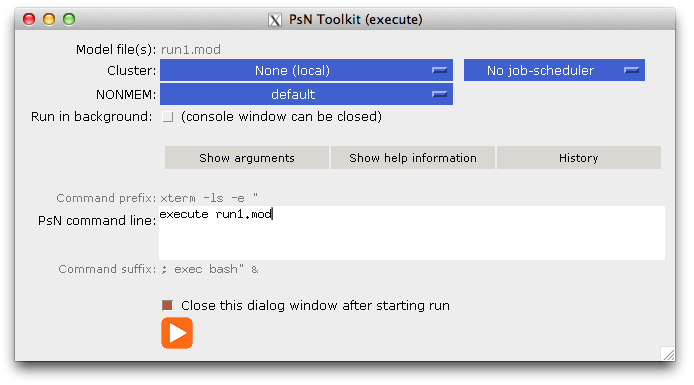
\includegraphics[scale=0.4]{images/fig2_psn_execute.png}
    \caption{PsN dialog window}
\end{figure}

\noindent Check that inside the folder created by PsN, a subfolder is created in which the
NONMEM process actually runs (\fname{/NM\_run1}). In Pirana, PsN folders are
hidden by default, as they may quickly clutter the model overview. To
unhide them again, select either “PsN folders” or “All folders” from
the folder selector (button 7 in figure 1). Many additional arguments
can be supplied to PsN commands to customize how PsN runs the NONMEM
model, e.g.: 

\begin{lstlisting}
execute run1.mod -dir=test1 –retries=3 -parafile=mpi6.pnm 
  –nm_version=nm72
\end{lstlisting}

\noindent which will run model run1.mod in the folder \fname{/test1}. PsN is
also instructed now to run using NONMEM version 7.2, parallelized
using MPI (specified in configuration file mpi6.pnm), and to retry
three times if the model doesn’t converge in the initial run, each
time changing the initial estimates of the parameters. A list of all
available arguments including help information is available from the
PsN dialog window in Pirana (figure 2), which is similar to using the
\command{-h} and \command{–help} arguments on the command line. In the PsN configuration
file (\fname{psn.conf}), a list of default arguments can be supplied as well,
so commonly used arguments do not have to be repeated on the command
line.

\subsubsection{Results evaluation} After estimation has completed,
refresh the Pirana main overview again. Basic results are now shown
for the run, such as the objective function value (OFV), whether
minimization was successful (S), and whether the covariance step was
successful (C). If the run was successful, PsN will automatically copy
back the results file (\fname{run1.lst}) and the produced output tables
(sdtab1, patab1) to the parent folder, which are then parsed by Pirana
upon refreshing. Select the model again, and now select the \action{Estimates
tab} from the right section of the Pirana window (11 in figure 1). The
right section will then show the parameter estimates for this run. A
more detailed overview that will e.g. show full random effect blocks
can be opened from here. Create a run summary in Word format
(alternatives are HTML, plain text or LaTeX), from the \action{menu $\rightarrow$ Results
$\rightarrow$ Run Reports $\rightarrow$ Word}. 

Diagnostic plots are a main decision tool in pharmacometric model
development, in which a distinction can be made between residual-based
diagnostics (goodness of fit plots based e.g. on residuals plotted
versus time or model predictions), and simulation-based diagnostics
(e.g. visual predictive checks, VPC). Obviously no strict rule should
be applied here, but in our experience residual-based diagnostics are
more useful in the first stages of model development, while
simulation-based diagnostics are more useful in the latter stages of
model development. Depending on what part of the model is diagnosed,
different diagnostic plots will be useful, and most likely no single
plot will suffice to evaluate model fit. Suggestions for diagnostic
plots for specific model parts are shown in table 1. Note that this
list is not exhaustive, and in addition, more specific plots may be
required for appropriate diagnosis.

\begin{figure}[H] \centering
    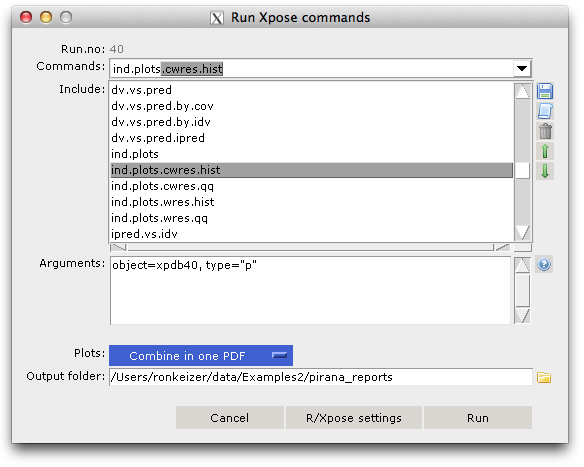
\includegraphics[scale=0.4]{images/fig3_xposeGUI.png}
    \caption{Xpose dialog window}
\end{figure}

For the current analysis, we will first have a look at some basic,
residual-based goodness of fit plots. A general model diagnostic is
the plot of weighted residuals versus time, or versus model
predictions. For models run with the conditional estimation method
(FOCE), it is most appropriate to use conditional weighted residuals
(CWRES, [10]). 

\begin{landscape}
\begin{table}[ht]
\caption{Suggested diagnostic plots in Xpose for PK development}
\vspace{10pt}
\footnotesize
\begin{tabular}{ p{4cm} p{12cm} }
Residual error model &
\begin{itemize}
\item Individual weighted residuals versus individual predictions (absval.iwres.vs.ipred)
\item Distribution / qq-plot of IWRES (iwres.dist.hist/qq)
\item In case of shrinkage: CWRES (cwres.dist.hist) or IWRESnpde 
\item Autocorrelation in residuals (autocorr.iwres)
\end{itemize} \\
Between subject variability model &
\begin{itemize}
\item Distribution / qq-plot of EBE’s (parm.hist.hist/qq)
\item In case of shrinkage: distribution of EBE$_{npde}$
\item Correlation between parameters (parm.splom)
\end{itemize} \\
Inter-occasion variability model &
\begin{itemize}
\item EBE parameter values vs occasions
\item Distribution / qq-plot of EBE (parm.dist.hist/qq)
\item In case of shrinkage: distribution of EBE$_{npde}$
\end{itemize} \\
Absorption model] &
\begin{itemize}
\item Individual profiles (ind.plots)
\item CWRES vs time after dose (cwres.vs.tad)
\item Individual g.o.f. plots (dv.vs.pred.ipred.by.idv)
\item Distribution of absorption parameters (ka, MTT, F) (parm.hist)
\end{itemize} \\
\end{tabular}
\end{table}
\end{landscape}

\begin{landscape}
\footnotesize
\begin{tabular}{ p{4cm} p{12cm} }
Disposition model & 
\begin{itemize}
\item Residuals versus time (cwres.vs.idv)
\item Individual profiles (ind.plots)
\item VPC (xpose.VPC)
\end{itemize} \\
Covariates &
\begin{itemize}
\item Parameter (EBE) vs covariate (parm.vs.cov)
\item In case of shrinkage: EBEnpde vs covariate 
\item G.o.f. plots by covariate (dv.pred.vs.idv.by.cov)
\item Correlations between covariates (cov.splom)
\item Influential individuals (dOFV.vs.id)
\item VPC stratified by covariate (xpose.VPC)
\item VPC with covariate as IDV (xpose.VPC)
\end{itemize} \\
\end{tabular}
\end{landscape}
\normalsize

\noindent Use the Xpose GUI within Pirana to create these plots:
\action{select model $\rightarrow$ right click $\rightarrow$ Xpose
$\rightarrow$ Xpose GUI}. Add the plot \command{cwres.vs.pred} and \command{cwres.vs.idv}
to the list of plots, and possibly some additional goodness-of-fit
plots (a list of useful Xpose plots is given in table 2). In these
plots you should observe an obvious pattern in the residuals. It may
not be obvious immediately what is the cause of the misspecification,
but a look at the individual plots (\command{ind.plots}) probably gives more
insight: the model seems to be missing the bi-phasic nature of the
observed data. Therefore, in the next step we will add distribution of
drug into a peripheral compartment to our PK model, but first we will
briefly discuss how to keep track of model development

Besides the Xpose GUI, there are several alternative ways of creating
diagnostic plots from Pirana:

\begin{itemize}
\item DataInspector: a quick and flexible method for creating
  diagnostic plots based on NONMEM output, or checking input
  datasets. Select the DataInspector for \fname{run1.mod} (\action{right click
  $\rightarrow$ Model $\rightarrow$ Open DataInspector}). Pirana will
  ask you now which input- or ouput file to open, choose the file
  sdtab1. In the DataInspector window, the variables on the x- and
  y-axis can be easily changed to any variable in the dataset, and
  filters can be applied on patient ID, or on any other variable. From
  this window, R-code can be generated that will recreate the same
  graph in R.
\item R script library: Pirana comes bundled with a library of
  diagnostic R scripts, which can be run automatically from
  Pirana. Select a model and select the one of the R-scripts from the
  Scripts Tab, e.g. \action{Basic GOF $\rightarrow$ DV vs IPRED}, and then
  select Run script from the buttons above the list. The requested
  plot will be created in a PDF document and opened. Created plots
  will be listed in the “Reports” tab (10 in figure 1). The standard
  scripts bundled with Pirana can be extended and customized easily,
  but that is beyond the scope of this tutorial. Please refer to the
  manual and default scripts for guidance.

\item Xpose menu system in R: The Xpose menu system can be started
  from Pirana (\action{right click $\rightarrow$ Xpose $\rightarrow$ Start
  Xpose menu in R}), or manually from an R session by
  invoking:
  \begin{lstlisting}
    library(xpose4)
    xpose4()
  \end{lstlisting}

  Xpose will then ask for the run number, which is used to determine
  which tables to import. Note that to use Xpose, NONMEM needs to be
  instructed to output tables that adhere to a specific naming and
  structure (see online materials table I, or the Xpose website). If
  you didn’t use the Pirana model wizard to create the tables, add
  them manually in the NONMEM model file, using e.g.:

\begin{lstlisting}
$TABLE ID TIME IPRED IWRES EVID MDV 
       NOPRINT ONEHEADER FILE=sdtab1
\end{lstlisting}

From the Xpose menu system, goodness-of-fit plots can
be created, e.g. browse to 

\begin{lstlisting}
4: Goodness of fit plots
2: Basic goodness of fit plots
\end{lstlisting}

\end{itemize}

\begin{landscape}
\begin{table}[ht]
\caption{Commonly used arguments for Xpose functions}
\vspace{10pt}
\footnotesize
\begin{tabular}{ p{3.1cm} p{9cm} p{4.5cm}}
\textbf{Function} & \textbf{Description} & \textbf{Commonly used arguments} \\ 
basic.gof & Compound plot of basic goodness-of-fit plots & use.log, force.wres\\
y-var.vs.x-var & General diagnostics functions: y-var can be one of dv, pred, ipred, iwres, cwres, wres. x-var can be any of pred, ipred, idv. Add “.by.cov” or “.by.idv” to the command to split the plot by covariate or by individual. & abline, smooth\\
ind.plots & Plots of dv, pred and ipred versus time, split by individual. & y.vals, layout\\
xpose.VPC & Visual predictive check (uses PsN output folder) & VPC.info, VPCtab, PI.ci, PI.real, type\\
xpose.VPC.categorical & Visual predictive check for categorical data & level.to.plot, max.plots.per.page\\
xpose.VPC.both & Visual predictive check for continuous and categorical data (e.g. BLOQ data) & See above\\
autocorr.cwres & Plot cwrest+1 vs cwrest to check for autocorrelation in residuals & type, smooth, ids\\
parm.hist / parm.qq & Plot distributions / qq-plots of model parameters & onlyfirst\\
parm.vs.parm & Plot model parameter versus model parameters & onlyfirst, abline, smooth\\
parm.vs.cov & Plot parameters and eta’s versus covariates to check for correlation & onlyfirst, smooth\\
xpose.gam & Generalized Additive Models (covariate model building tool) & parnam, covnams, start.mod\\
basic.model.comp & Compare basic goodness-of-fit plots between two models & object.ref\\
kaplan.plot & Visualizes data and VPC from survival models & x, y, id, data, by \\
\end{tabular}

\bigskip

\textit{
\noindent For most functions listed above, the following general arguments are useful: object (which Xpose database to use), main (plot title), inclZeroWRES (include values where WRES is zero).\\
\noindent In R, help information for functions can be obtained by giving the command ?<function>, where <function> is the  desired R/Xpose function. \\
\noindent Abbreviations: dv = dependent variable, idv = independent variable, (c/i)wres: (conditionally / individual) weighted residuals. pred = population predicitions, ipred = individual predictions.
}
\end{table}
\end{landscape}

\subsubsection{Model management in Pirana}
In M\&S projects in both academia and industry, it is essential to
keep track of the model development history. Pirana and PsN offer a
tool to aid the modeler with this through the run record. The run
record entails a standardized way of keeping track of model meta
information such as the “parent” model, a description and/or a label
for the model, and other information about the model components. We
consider it good modeling practice to create a new model file for
every change that is made to a model. 

Duplicate the first model in Pirana (\action{right click on \fname{run1.mod} 
$\rightarrow$ File actions $\rightarrow$ duplicate}). In the dialog
that will open up, \fname{run2.mod} is suggested as new model file name, and
we can select which model is the reference model for this model
(\fname{run1.mod}), and optionally update the initial estimates with the
parameter estimates from the reference model. The model description
and other meta-information is stored in the model file itself using
the run record syntax (also see the userguide for the run record on
the PsN website). Pirana can show the main model overview as a list or
as a tree (button 6 in fig 1), and can export a copy of the run record
to various formats including comma separated (\fname{csv}) files, HTML files
and Word documents (\action{Results $\rightarrow$ Run records}), or create an
interactive visualization of the model development tree or “visual run
record”[11] like shown in figure 4 (\action{Results $\rightarrow$ Run records
$\rightarrow$ Visual run record}).

\begin{figure}[H] \centering
    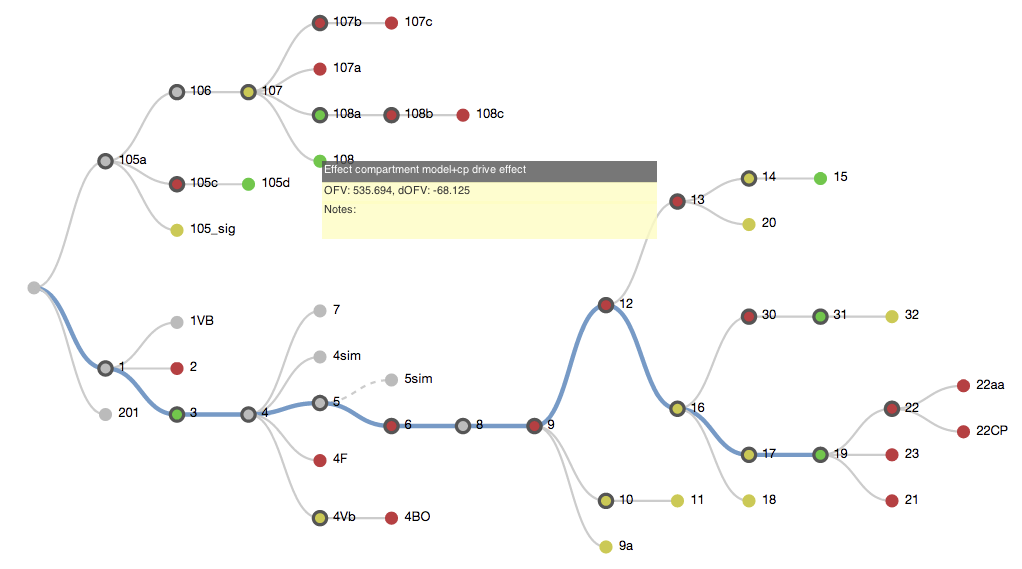
\includegraphics[scale=0.3]{images/fig4_vrr.png}
    \caption{Visual Run Record}
\end{figure}

After duplication, the model \fname{run2.mod} will be shown in the model
overview, and opened in the editor, where we will now add a peripheral
compartment to the model error model: change \$SUBROUTINE to use ADVAN3
and TRANS4, change the parameter V into V1, and add to \$PK: 

\begin{lstlisting}
Q = THETA(3)
V2 = THETA(4)
\end{lstlisting}

\noindent Of course, initial estimates for the intercompartmental distribution
(Q) and peripheral compartment (V2) have to be specified as well in
\$THETA. For now we chose to run this model without IIV on these
parameters. Run this model using execute, evaluate the drop in
objective function, and compare the diagnostic plots for run2 to those
made for run1. You should encounter a considerable drop in the
objective function value, and find that the diagnostic residual plots
show much improved model fit. 

Next, we will diagnose the residual error model, for which an
important diagnostic plot is that of absolute individual weighted
residuals ($|$IWRES$|$) versus individual predictions (IPRED). For a true
model, the distribution of absolute residuals should be similar over
the whole range of the x-axis variable. If a homoscedastic error
structure (additive error) was implemented in \fname{run1.mod} and \fname{run2.mod},
the plot will show larger residuals at higher individual 
predictions. This should therefore lead you to conclude that a
heteroscedastic (combined proportional and additive) error model
should provide a better description of the data. Therefore, create a
new model (run3.mod) based on run2.mod and implement a combined error
model using e.g.: 

\begin{lstlisting}
Y = IPRED * (1+EPS(1)) + EPS(2)
W = SQRT(IPRED**2*SIGMA(1,1)**2 + SIGMA(2,2)**2)
IWRES = (DV-IPRED)/W
\end{lstlisting}

\noindent It must be noted that the plot mentioned above is only
informative at low ε-shrinkage (as a rule-of-thumb, at $\epsilon$-shrinkage $>
~5\%$ this plot loses informativeness).[12] In cases of higher
shrinkage, plots of CWRES versus individual predictions (IPRED), or
IWRES$_{npde}$ [13] versus IPRED are more informative. The diagnostic plots
as well as the significant drop in OFV indicate that the combined
error model provides better fit. 

\subsubsection{Covariate model}
The dataset \fname{pktab1} contains three continuous covariates: weight (WT),
creatinine clearance (CRCL), AGE, and two binary covariates: SEX and
study center (CENT). Since the number of covariates is low (5), one
might choose to test these covariates manually. However, in the next
step of this tutorial we will perform stepwise covariate modeling
(scm) in PsN, to demonstrate this automated method. In the first phase
of the scm, covariates are added to the base model in a stepwise
fashion based on statistical significance (decrease in OFV). In a
second “backward elimination” phase, covariates are then removed from
the final model obtained in the first phase, if removal of the
covariate does not result in significantly worse fit. The backward
step is typically done at a higher significance level. Like all PsN
tools, the scm can be run from the command line or from Pirana, in a
similar way as done before for execute. However, the scm tool requires
that a configuration file is created first. Several examples of
configuration files are available on the PsN website, but here we will
create one using the wizard in Pirana (\action{Tools $\rightarrow$ Wizards
$\rightarrow$ scm configuration file}).  Create a configuration file,
with the filename \fname(psp.scm), in which all covariates are tested on both
CL and V1, at a significance level of 0.1 (forward step) and 0.05
(backward step) and restrict the analysis to linear relationships (set
the relationships argument to “1,2”). Check that the correct
covariates are included; the ones shown in the wizard are only
placeholders. If you’re not sure on the correct syntax of the scm
file, please have a look at the provided annotated configuration file
(psp.scm in the on-line appendix). Before starting the scm, duplicate
run3.mod to run4.mod, and remove any \command{\$TABLE} records that are
present. Start the scm from the PsN dialog window using this command:

\begin{lstlisting}
scm psp.scm –model=run4.mod
\end{lstlisting}

\noindent After the scm has completed, PsN will compile an output file
called \fname{scmlog.txt} in the scm folder. Open this file and interpret the
information, it holds the results for all tests performed in the scm
and shows how the final covariate model was constructed. You should
find that 4 covariate relationships are significant: CRCL on CL, WT on
CL, WT on V, and SEX on V. This will be our “final model” from the
covariate model-building step. If you did not find these results,
compare your results with those provided in the on-line
appendix.

More elaborate covariate model building techniques based on the scm
are available in PsN as well, such as the cross-validated scm
(\command{xv\_scm})[14], and the bootstrap of the scm (\command{boot\_scm})[15]. These tools
provide more details on the predictive ability of the model, and on
selection bias and expected covariate model size, respectively. They
can also be run on linearized versions of the model, to reduce the
computational workload.[16] Other covariate modeling tools that are
available in PsN include the lasso[17] and the fixed random effects
model (FREM, [18]), while in Xpose the gam and bootstrap of the gam
(bootgam) are implemented [6]. All of these methods have certain
advantages and drawbacks, which are however beyond the scope of this
article.

\subsubsection{Final model}
If the scm completed successfully, you will find a folder called
\fname{final\_models} inside the scm folder created by PsN. Inside that folder,
locate the final model with included covariate relations and copy that
to the main model folder, renaming it to \fname{run5.mod}. We will use this
model to perform some more elaborate diagnostic evaluation, i.e. we
will get bootstrap estimates for our parameters and create a VPC. So
first open the PsN bootstrap dialog window (\action{Right click $\rightarrow$
PsN $\rightarrow$ Model diagnostic $\rightarrow$ bootstrap}). A
required argument to the bootstrap command is the –samples argument,
which specifies how many bootstrap samples should be drawn. More
samples will make the bootstrap estimates and percentile estimates
more precise, however at the expense of increased computation
times. The recommended number of samples for an analysis will depend
on what statistic is desired by the modeler. For obtaining bootstrap
means of the parameter estimates, 100 samples may be enough, but to
obtain accurate 5th and 95th percentiles, 1,000 or more are required
to obtain precise estimates. After the bootstrap is finished (on a
single core, a bootstrap of 200 samples may easily take an hour for
this model), the results from the bootstrap are available in the
bootstrap folder, in the files \fname{raw\_results\_run5.csv} and
\fname{bootstrap\_results.csv}. Open these files and interpret the output: are
the parameters estimated with adequate precision? In Pirana, select
the bootstrap folder created by PsN and run the R-script to create
plots of parameter distributions (\action{Scripts tab $\rightarrow$ PsN
$\rightarrow$ Bootstrap results}), which facilitates evaluation and
interpretation of these bootstrap results. 

Earlier in this tutorial we presented how basic goodness-of-fit plots
can be created in Pirana and Xpose. Now we will use all three tools to
create a visual predictive check (VPC) of the final model
(run5.mod). A VPC is an internal validation tool, i.e. it shows how
well the model predicts the data on which the model was
conditioned. It visualizes the median model prediction, the
variability between patients and within patients (5th and 95th
percentiles), and the uncertainty around the predicted
percentiles.[19] Before we create a VPC, we would like to stress a few
points. Firstly, in VPCs it is important to show the uncertainty
around the model predicted percentiles, instead of presenting only
lines indicating the point estimates of the percentiles. Signs of
model improvement are when the confidence areas of the simulated
percentiles encompass more of the observation percentiles, but also
when the confidence intervals themselves are shrinking (while still
encompassing the observation percentiles).  Furthermore, since the VPC
shows summary statistics (percentiles) of observations and predictions
for binned data, the “binning method is an important consideration. To
avoid inflation of the uncertainty around the summary statistics, each
bin should contain an adequate amount of observations. A quick
rule-of-thumb is that there should not be more bins than the number of
observations per individual. PsN currently incorporates several
binning approaches: manual bin specification (\command{-bin\_array=x,y,z,etc}),
binning into an equal number of datapoints per bin (\command{-bin\_by\_count=1
–no\_of\_bins=\#}), or spacing the bins equally over the x-axis
(\command{-bin\_by\_count=0}, \command{-no\_of\_bins=\#}). Importantly, binning across a large
variability in dose and/or influential covariates can diminish the
diagnostic value of a VPC. One approach to overcome this is to
stratify the VPC by the covariate, but this is not always possible
e.g. due to limited data per stratum. Also when data arises from
studies with adaptive designs (e.g. dose adjustments), VPCs are
misleading unless the adaptation protocol is included in the
model. The prediction-corrected VPC (pcVPC) offers a solution to these
problems while retaining the visual interpretation of the traditional
VPC.[20] pcVPCs can be constructed by adding the argument \command{–pred\_corr}
to the PsN VPC command.

\begin{figure}[H] \centering
    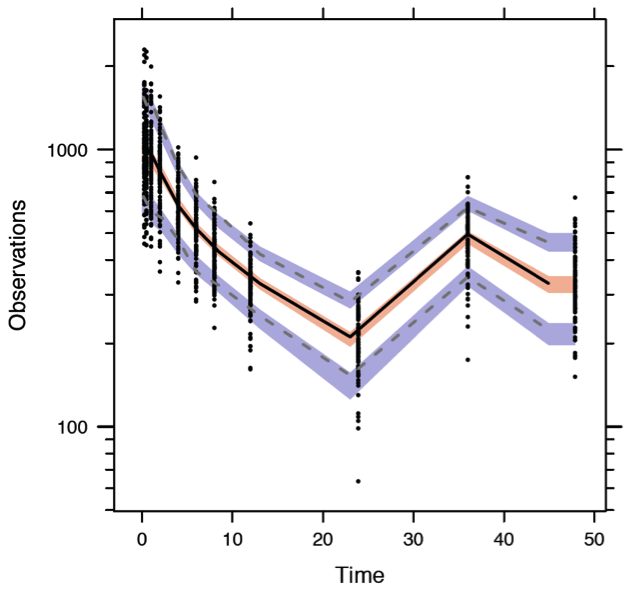
\includegraphics[scale=0.8]{images/fig5_vpc.png}
    \caption{Visual Predictive Check (vpc)}
\end{figure}

VPCs can be made in Pirana using the PsN dialog window (\action{right click
$\rightarrow$ PsN $\rightarrow$ model evaluation $\rightarrow$ VPC}),
or from the command line. As discussed above, essential arguments to
pass to the VPC are the number of samples and the binning
method. Increasing the number of samples will increase the accuracy of
the summary statistics for the simulation and their uncertainty
interval (but it will not decrease the uncertainty interval
itself). Start the VPC tool using:

\begin{lstlisting}
  vpc –samples=500 –no\_of\_bins=8 –bin\_by\_count=1 run5.mod
\end{lstlisting}

The first of the two NONMEM runs that are started will only output a
table with the necessary (observation) data for the VPC, it does not
perform parameter estimation. The other model runs repeated Monte
Carlo simulations of the model, using the same dataset design as the
original. After the two NONMEM runs have finished, PsN will process
the output, bin the simulated and observed data, calculate the
percentiles and confidence intervals for each bin, and export a
csv-file with the summary statistics. This csv-file can then be
processed by Xpose and turned into a VPC-plot, which can be automated
from Pirana using the Xpose GUI as described before, or using the R
scripts library. Both approaches will create and open a pdf-file with
the VPC (see example in figure 5). Using the latter approach this is
done as follows: select the VPC-folder created by PsN, and open the
Scripts tab on the right. In the list of R scripts, choose \action{Xpose
$\rightarrow$ VPC $\rightarrow$ Basic\_log\_y.R}. A pdf-file with the VPC
will be generated and opened from Pirana. As an exercise, try to
create the same plot using the Xpose GUI in Pirana as well: select the
model in the main overview, and \action{right click $\rightarrow$ Xpose
$\rightarrow$ Xpose GUI}. Since only limited space is available for
this tutorial we will not demonstrate other diagnostics. We will
however create a run record of the model development: in the menu bar
click \action{Results $\rightarrow$ Run records $\rightarrow$ Detailed run
record (csv)}. This will create and open a csv-file containing run
numbers, descriptions, other meta-information and run results. If the
file does not open automatically, please look it up in the “Files” tab
on the right and double click it. As a final step in our PK model
development, select the final model again and bundle that model file,
the associated result files and output files and the VPC folder into a
zip-file (\action{Right click $\rightarrow$ File actions$\rightarrow$ Compress
to zip-file}). Also create a bundled report of the goodness-of-fit
plots for the final model (in the Reports tab select the desired pdf’s
and click \action{Bundle into... $\rightarrow$ $<$output format$>$}). 

\subsubsection{Additional features}
For all three software tools presented here, we have only scratched
the surface of possibilities. The reader is encouraged to explore more
advanced functionality using the documentation available on the
respective websites. We will highlight a few examples of more advanced
features for the three programs below.

\begin{description}
\item[PsN] the simulation and re-estimation (\command{sse}) tool can be used to
  evaluate trial designs, e.g. to evaluate whether model parameters
  can be estimated with adequate precision under the intended or
  alternative experimental designs or with alternative models. It is
  also useful for evaluating fundamental modeling aspects, e.g. to
  evaluate how model diagnostics perform under given designs. Another
  interesting tool for design evaluation, specifically for the
  calculation of study power and number of study subjects required, is
  Monte Carlo Mapped Power (\command{mcmp}).[21] In this tool, which is also
  based on simulation and re-estimation, the individual objective
  function values calculated in NONMEM are exploited to evaluate
  designs in a more rapid way than using sse. Case deletion
  diagnostics (\command{cdd}) is a tool that can be useful in the final stages
  of model development, to investigate whether model fit depends more
  heavily on particular strata of the dataset. The most important PsN
  functions are listed in table 3.
\item[Xpose] In this tutorial we showed how to create goodness-of-fit
  plots from the Xpose menu system, and from the Xpose interface in
  Pirana (VPC). However, the most efficient way to use Xpose,
  especially when doing repetitive jobs, is to use scripts to create
  the desired goodness-of-fit plots. A list of useful Xpose functions
  is given in table 2, while a more complete overview of functions and
  example scripts (“bestiarium”) is available on the Xpose
  website. The default plots in Xpose can be extended and modified in
  various ways. Firstly, most Xpose functions take arguments that
  alter the implementation of the plot. The looks of the plots can
  also be changed by directly passing lattice arguments to the Xpose
  function. Secondly, the input variables can be altered easily to
  allow creation of non-default plots. E.g. to create a plot of a
  covariate METAB vs IDV instead of DV vs IDV we can ‘trick’ Xpose
  into using METAB as DV while maintaining the plot
  characteristics:
\begin{lstlisting}
> change.xvardef(xpdb, "dv") <- c("METAB")
> xplot <- dv.vs.idv(xpdb)
> print(xplot)
\end{lstlisting}

\noindent Finally, since Xpose is an open source R module, it is possible to
modify the Xpose functions directly, if further modifications are
required.

\item [Pirana] a model translator is included that can translate
any NONMEM model (written in an NM-TRAN ADVAN subroutine), to
differential equation code for R (using deSolve library), Berkeley
Madonna (software dedicated to ODE simulations), or Matlab / PopED
[22]. Note that many functions in Pirana can be extended and
customized by the user, such as the R-scripts library and the
wizards. Pirana can also be used for modeling on remote clusters
(through ssh-connections), and has native support for SGE, Torque and
Condor job schedulers.

\end{description}

\begin{landscape}
\begin{table}[ht]
\caption{Commonly used PsN tools}
\vspace{10pt}
\footnotesize
\begin{tabular}{ p{3.1cm} p{6cm} p{7.5cm}}
\textbf{Tool command} &  \textbf{Description} & \textbf{Commonly used arguments}\\
execute & Run a model in NONMEM & -retries –picky –model\_dir\_name \\
VPC & Visual predictive check & -samples -bin\_by\_count –no\_of\_bins –bin\_array –dv -idv\\
bootstrap & Run a bootstrap & -samples –stratify\_on \\
cdd & Case deletion diagnostics & -samples –case\_column \\
sse & Simulation and (re-)estimation & -samples –alternative\_models –no-estimate\_simulation \\
mcmp & Monte Carlo Mapped power & -n\_bootstrap –start\_size –increment -df \\
scm & Stepwise covariate modeling & -config\_file –model \\
xv\_scm & Cross-validated stepwise covariate modeling & -config\_file –max\_steps -splits \\
boot\_scm & Bootstrap of stepwise covariate modeling & -config\_file -samples –dummy\_covariates -run\_final\_models \\
llp & Log-Likelihood profiling and maximum-likelihood parameter estimates & -ofv\_increase –thetas –omegas –max\_iterations \\
psn\_options & Shows all general PsN options & -nm\_version -verbose \\
update\_inits & Updates initial estimates based on a NONMEM output file from a previous run & -from\_model –output\_model \\
lasso & the Lasso (covariate modeling) & -relations –lst\_file \\
mimp & Multiple imputation (missing data method) & -base\_model –reg\_model –mi\_model -imputations \\
General options* & Applies to every PsN tool  & -clean \\

\end{tabular}

\bigskip

\textit{
\noindent For each tool, the arguments –h and –help show a list of arguments and a detailed description of the arguments, respectively. \\
\noindent Note that arguments can also be set in the psn configuration file. 
In that case they don’t have to be specified again on the command line.
}

\end{table}
\end{landscape}

\section{Conclusion} In this tutorial we presented a modeling
workbench that incorporates three tools, which in our view make M\&S
with NONMEM more powerful, more efficient and easier to perform. It is
our intention to implement all new modeling techniques and diagnostics
developed within our group into PsN, Xpose and/or Pirana, so new
versions are expected to be released on a regular basis.


\subsubsection{Conflict of Interest}RJK is owner of Pirana Software \& Consulting
BV, which provides commercial licensing of Pirana. MOK and
AH have no conflicts of interests.

\subsubsection{Acknowledgements}
The researchers in the Pharmacometrics Research Group are acknowledged
for their input on the use of diagnostics in model
development.


\subsection*{References}
\scriptsize 
\begin{enumerate}
\item Sheiner LB, Beal SL. Evaluation of methods for estimating
  population pharmacokinetics parameters. I. Michaelis-Menten model:
  routine clinical pharmacokinetic data. Journal of pharmacokinetics
  and biopharmaceutics [Internet] 1980 [cited 2012 Aug 3];8(6):553–71.

\item Stone JA, Banfield C, Pfister M, Tannenbaum S, Allerheiligen S,
  Wetherington JD, et al. Model-based drug development survey finds
  pharmacometrics impacting decision making in the pharmaceutical
  industry. Journal of clinical pharmacology [Internet] 2010 [cited
  2012 Aug 3];50(9 Suppl):20S–30S.

\item Zandvliet AS, Schellens JHM, Beijnen JH, Huitema ADR. Population
  pharmacokinetics and pharmacodynamics for treatment optimization in
  clinical oncology. Clinical pharmacokinetics [Internet] 2008 [cited
  2012 Aug 3];47(8):487–513.

\item Lindbom L, Pihlgren P, Jonsson EN, Jonsson N. PsN-Toolkit--a
  collection of computer intensive statistical methods for non-linear
  mixed effect modeling using NONMEM. Computer methods and programs in
  biomedicine [Internet] 2005 [cited 2012 Jul 25];79(3):241–57.

\item Vlasakakis G, Comets E, Keunecke A, Gueorguieva I, Magni P,
  Terranova N, et al. White paper: Landscape on technical and
  conceptual requirements and competence framework in Drug / Disease
  Modeling \& Simulation. CPT:PSP (In press)

\item Jonsson EN, Karlsson MO. Xpose--an S-PLUS based population
  pharmacokinetic/pharmacodynamic model building aid for
  NONMEM. Computer methods and programs in biomedicine [Internet] 1999
  [cited 2012 Aug 3];58(1):51–64.

\item Keizer RJ, Van Benten M, Beijnen JH, Schellens JHM, Huitema
  ADR. Piraña and PCluster: a modeling environment and cluster
  infrastructure for NONMEM. Computer methods and programs in
  biomedicine [Internet] 2011 [cited 2011 Jul 12];101(1):72–9.

\item Byon W, Smith MK, Chan P, Tortorici MA, Riley S, Dai H, et
  al. Establishing Best Practices and Guidance in Population Modeling:
  an Industry Experience with a Population Pharmacokinetic Analysis
  Guidance. CPT:PSP (In press)

\item Beal S, Sheiner LB, Boekmann A, Bauer RJ. NONMEM’s User's
  Guides. Ellicott City, Maryland, USA.: ICON Development Solutions;
  10.  Hooker AC, Staatz CE, Karlsson MO. Conditional weighted
  residuals (CWRES): a model diagnostic for the FOCE
  method. Pharmaceutical research [Internet] 2007

\item Keizer RJ. The Visual Run Record: visualization of the model
  development history. In: Abstracts of the World Conference on
  Pharmacometrics. Seoul, South-Korea: 2012.

\item Karlsson MO, Savic RM. Diagnosing model diagnostics. Clinical
  pharmacology and therapeutics [Internet] 2007 [cited 2012 Aug
  3];82(1):17–20.

\item Keizer RJ, Harling K, Karlsson MO. Extended NPDE diagnostics for
  the between-subject variability and residual error
  model. PAGE. Abstracts of the Annual Meeting of the Population
  Approach Group in Europe. 2012;21:Abstr 2538.

\item Katsube T, Khandelwal A, Harling K, Hooker AC, Karlsson
  MO. Evaluation of Stepwise Covariate Model Building Combined with
  Cross-Validation [Internet]. In: PAGE. Abstracts of the Annual
  Meeting of the Population Approach Group in Europe. 2011. page Abstr
  2111.

\item Keizer RJ, Khandelwal A, Hooker AC, Karlsson MO. The bootstrap
  of stepwise covariate modeling. In: PAGE. Abstracts of the Annual
  Meeting of the Population Approach Group in Europe. Athens, Greece:
  2011. page Abstr 2161.

\item Khandelwal A, Harling K, Jonsson EN, Hooker AC, Karlsson MO. A
  fast method for testing covariates in population PK/PD Models. The
  AAPS journal [Internet] 2011 [cited 2012 Aug 2];13(3):464–72.

\item Karlsson MO. A full model approach based on the covariance
  matrix of parameters and covariates. PAGE. Abstracts of the Annual
  Meeting of the Population Approach Group in Europe. 2012;21:Abstr
  2455.

\item A Tutorial on Visual Predictive Checks [Internet]. [cited 2012
  Aug 3]; http://www.page-meeting.org/default.asp?abstract=1434

\item Bergstrand M, Hooker AC, Wallin JE, Karlsson
  MO. Prediction-corrected visual predictive checks for diagnosing
  nonlinear mixed-effects models. The AAPS journal [Internet] 2011
  [cited 2012 Jul 17];13(2):143–51.

\item Vong C, Bergstrand M, Nyberg J, Karlsson MO. Rapid sample size
  calculations for a defined likelihood ratio test-based power in
  mixed-effects models. The AAPS journal [Internet] 2012 [cited 2012
  Aug 3];14(2):176–86.

\item Nyberg J, Ueckert S, Strömberg EA, Hennig S, Karlsson MO, Hooker
  AC. PopED: An extended, parallelized, nonlinear mixed effects models
  optimal design tool. Computer methods and programs in biomedicine
  [Internet] 2012 [cited 2012 Aug 13]
\end{enumerate}

\normalsize